\documentclass{ctexart}
\usepackage{graphicx} % Required for inserting images
\usepackage{hyperref}
\usepackage{float}
\usepackage{listings}
\usepackage{xcolor}
\usepackage{multirow}
\usepackage{multicol}
\usepackage{booktabs}
\usepackage{amsmath}
\usepackage[letterpaper,top=2cm,bottom=2cm,left=3cm,right=3cm,marginparwidth=1.75cm]{geometry}

\hypersetup{
    colorlinks=true,
    linkcolor=blue,
    filecolor=blue,
    urlcolor=blue,
    citecolor=cyan,
}

\definecolor{codegreen}{rgb}{0,0.6,0}
\definecolor{codegray}{rgb}{0.5,0.5,0.5}
\definecolor{codepurple}{rgb}{0.58,0,0.82}
\definecolor{backcolour}{rgb}{0.95,0.95,0.92}

\lstdefinestyle{mystyle}{
    backgroundcolor=\color{backcolour},
    commentstyle=\color{codegreen},
    keywordstyle=\color{magenta},
    stringstyle=\color{codepurple},
    basicstyle=\ttfamily\footnotesize,
    breakatwhitespace=false,
    breaklines=true,
    captionpos=b,
    keepspaces=true,
    showspaces=false,
    showstringspaces=false,
    showtabs=false,
    tabsize=2
}
\lstset{style=mystyle}

\title{EIEN6023P:Lab1-组合逻辑实验}
\author{}
\date{}

\begin{document}

\maketitle

\section{实验目标}
\begin{itemize}
    \item 熟悉Verilog的语法
    \item 熟悉Vivado的使用
    \item 使用Verilog编写七段数码管译码器代码
    \item 使用Verilog编写八位二进制全加器代码
    \item 在FPGAOL平台上进行验证所编写的代码
\end{itemize}

%------------------------------%

\section{七段数码管}

\subsection{原理}

七段数码管由七个独立的发光二极管构成,编码分别为a-g,可以用来显示一个字符。FPGAOL所使用的Nexys4 DDR开发板包含两个4位7段数码管,数码管中的每个LED都可以被单独点亮。在Nexys4 DDR开发板上,每位7段数码管的所有LED采用共阳极连接方式,可以通过在管脚输出\underline{\textbf{逻辑0}}来点亮对应的LED,如图所示。

\begin{figure}[H]
    \centering
    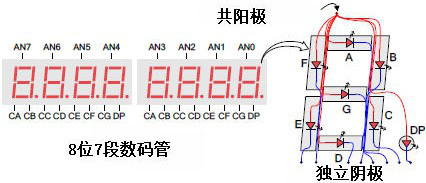
\includegraphics[width=0.8\textwidth]{lab1/1.png}
\end{figure}

可以注意到,如果每位7段数码管需要7个引脚来控制LED的亮灭,那么8位7段数码管一共需要$7*8=56$个管脚,这会消耗大量FPGA的IO资源。因此,Nexys4 DDR开发板采用多路复用的方式共享7段数码管的控制管脚,如图所示,CA-CG信号分别控制7段数码管上LED的亮灭,AN7-AN0信号分别控制8位7段数码管的亮灭。控制电路应使用扫描的方式来显示8位数字,一般情况下建议的刷新率为50Hz,对每一位LED的信号进行重复地、持续地、接连地驱动。通过控制每个LED的亮灭,每位7段数码管可以展示$2^7=128$种状态。

\subsection{实验内容}

在本节中,您将设计和实现一个七段数码管译码器的Verilog模块,该模块以4位二进制数字作为输入,并输出7位\underline{\textbf{低电平有效}}的信号以驱动7个发光二极管。4位二进制数字即十六进制数0-f,其对应的7段数码管a-g显示效果如图所示。

\begin{figure}[H]
    \centering
    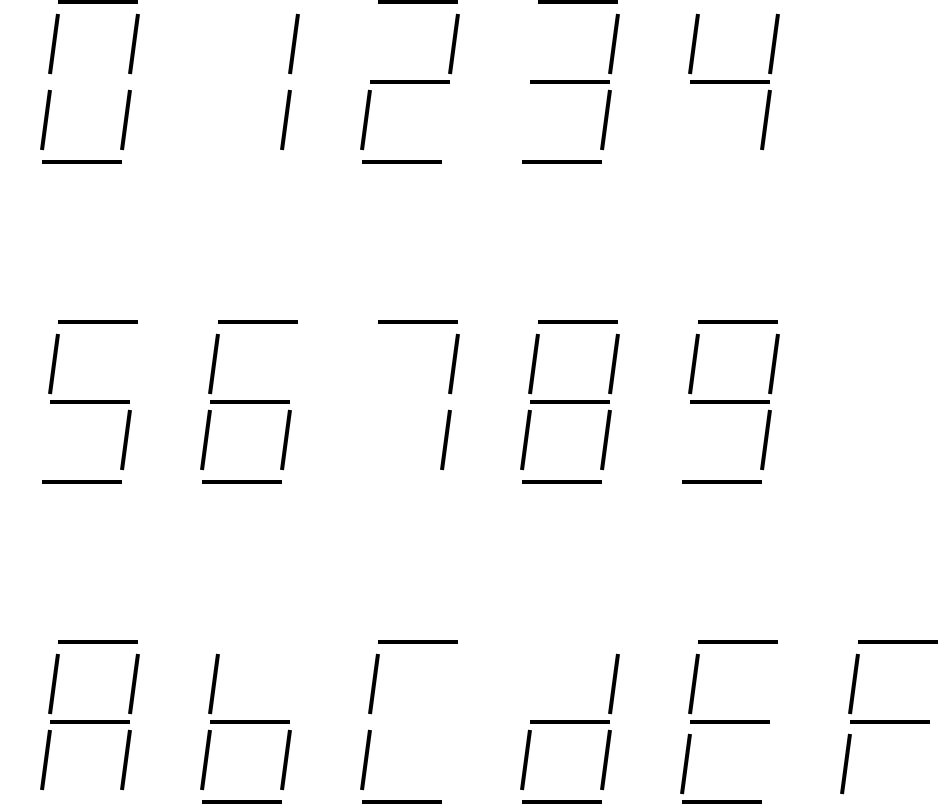
\includegraphics[width=0.4\textwidth]{lab1/2.png}
\end{figure}

\textbf{STEP1}:请编写4位二进制输入(A3-A0)和7位数码管驱动输出(a-g)之间对应的真值表。

\begin{table}[H]
    \centering
    \begin{tabular}{ c c c c c c c c c c c }
        \hline
        \multicolumn{4}{c}{Input} & \multicolumn{7}{c}{Output} \\
        \cmidrule(r){1-4} \cmidrule(r){5-11}
        A3 & A2 & A1 & A0 & a & b & c & d & e & f & g \\
        \hline
        0 & 0 & 0 & 0 & 0 & 0 & 0 & 0 & 0 & 0 & 1 \\
        0 & 0 & 0 & 1 & 1 & 0 & 0 & 1 & 1 & 1 & 1 \\
        \multicolumn{4}{c}{$\cdots$} & \multicolumn{7}{c}{$\cdots$} \\
        \hline
    \end{tabular}
\end{table}

\textbf{STEP2}:请使用卡诺图化简并写出各个输出项的逻辑表达式。
\begin{equation*}
    \begin{aligned}
        a &= A3' A2' A1' A0 + A3' A2 A1' A0' + A3 A2' A1 A0 + A3 A2 A1' A0 \\
        b &= \cdots  \\
        \cdots
    \end{aligned}
\end{equation*}

\textbf{STEP3}:请根据逻辑表达式编写Verilog代码,自行仿真验证。
\begin{lstlisting}[language=Verilog]
module seg_decoder (
    input [3:0] hex_in,
    output [6:0] seg_out // a-g
);
    // put your code here.
endmodule
\end{lstlisting}

%------------------------------%

\section{八位全加器}

\subsection{原理}

一个一位二进制全加器结构如下图所示,a与b为两个加数输入,c[i-1]为前一个加法器的进位输入,s为当前加法器的结果输出,c[i]为当前加法器的进位输出。该加法器执行的逻辑功能即:$\{c_i,s\}=a+b+c_{i-1}$。

\begin{figure}[H]
    \centering
    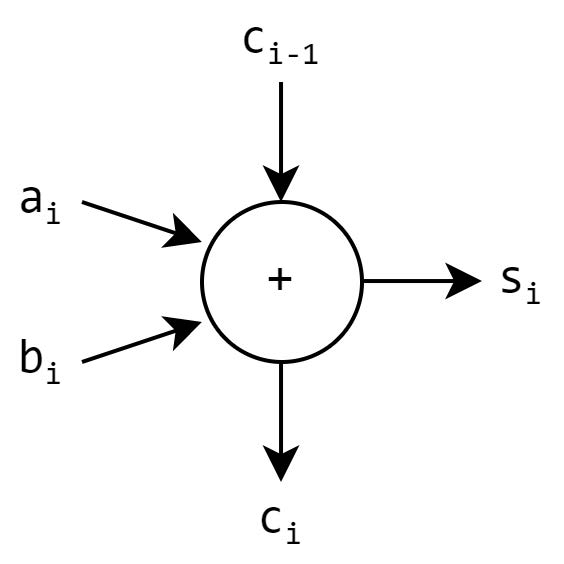
\includegraphics[width=0.2\textwidth]{lab1/3.jpg}
\end{figure}

现在我们拥有了一个一位二进制全加器,可以通过级联多个全加器来组成高位宽的加法器。根据进位信号的连接方式,我们可以将加法器分为两种:串行进位加法器与并行进位加法器。

\subsubsection*{串行进位加法器}

串行进位加法器又称为波纹进位加法器,其结构如下图所示。加数的每一位连接到对应的全加器的输入端口上,各个全加器之间的进位输入输出首位依次相连,进位信号依次传输,全加器的输出端口对应加法结果的每一位。由于每一个加法器的结果输出依赖于前一个加法器的进位输出,会形成较长的关键路径,导致运算速度变慢。

\begin{figure}[H]
    \centering
    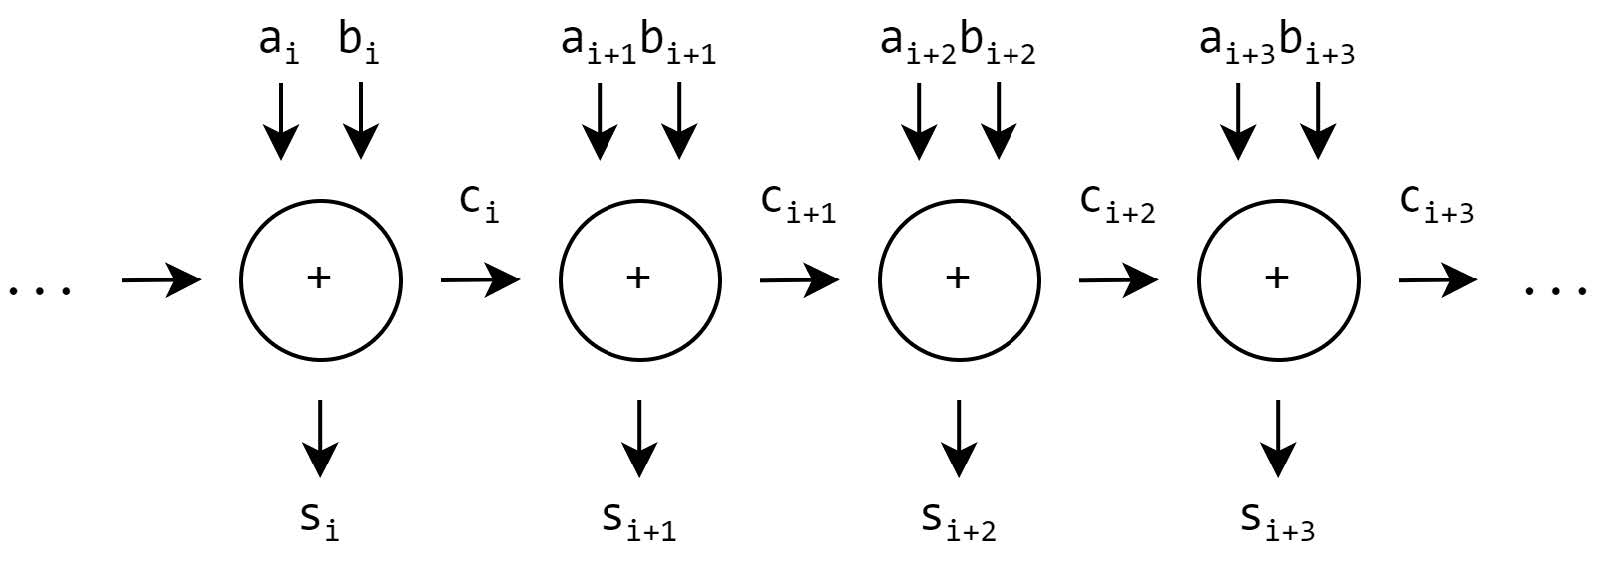
\includegraphics[width=0.6\textwidth]{lab1/4.jpg}
\end{figure}

\subsubsection*{并行进位加法器}

并行进位加法器又称为超前进位加法器,其结构如下图所示。其增加了专用的进位逻辑来直接输出进位信号给各个一位二进制加法器,进位逻辑经过更少的门电路来输出进位信号,因此可以加快计算速度。但当计算位宽较大时,会显著增加进位逻辑的复杂度。

\begin{figure}[H]
    \centering
    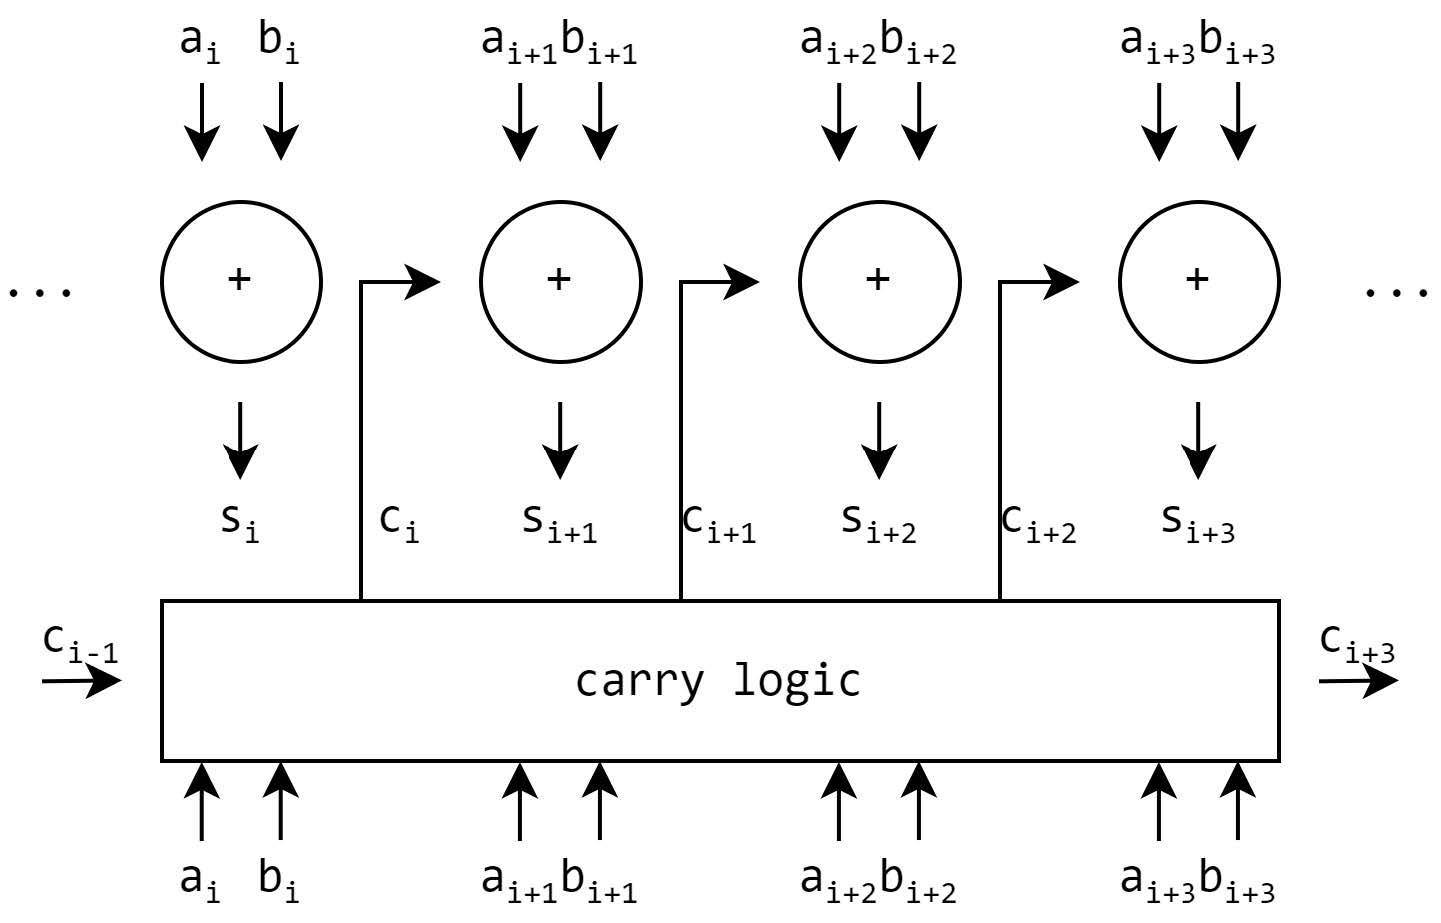
\includegraphics[width=0.55\textwidth]{lab1/5.jpg}
\end{figure}

\subsubsection*{混合进位加法器}

为了解决串行进位加法器的计算速度慢与并行进位加法器的设计复杂度高的问题,混合进位加法器被设计并应用,其结构如图所示。其采用了“组内并行、组间串行”的连接方式,增加计算速度的同时又不至于增加过多的设计复杂度。如果需要搭建位宽更高的全加器,则可以使用层次化的进位逻辑,这里不再扩展细述。

\begin{figure}[H]
    \centering
    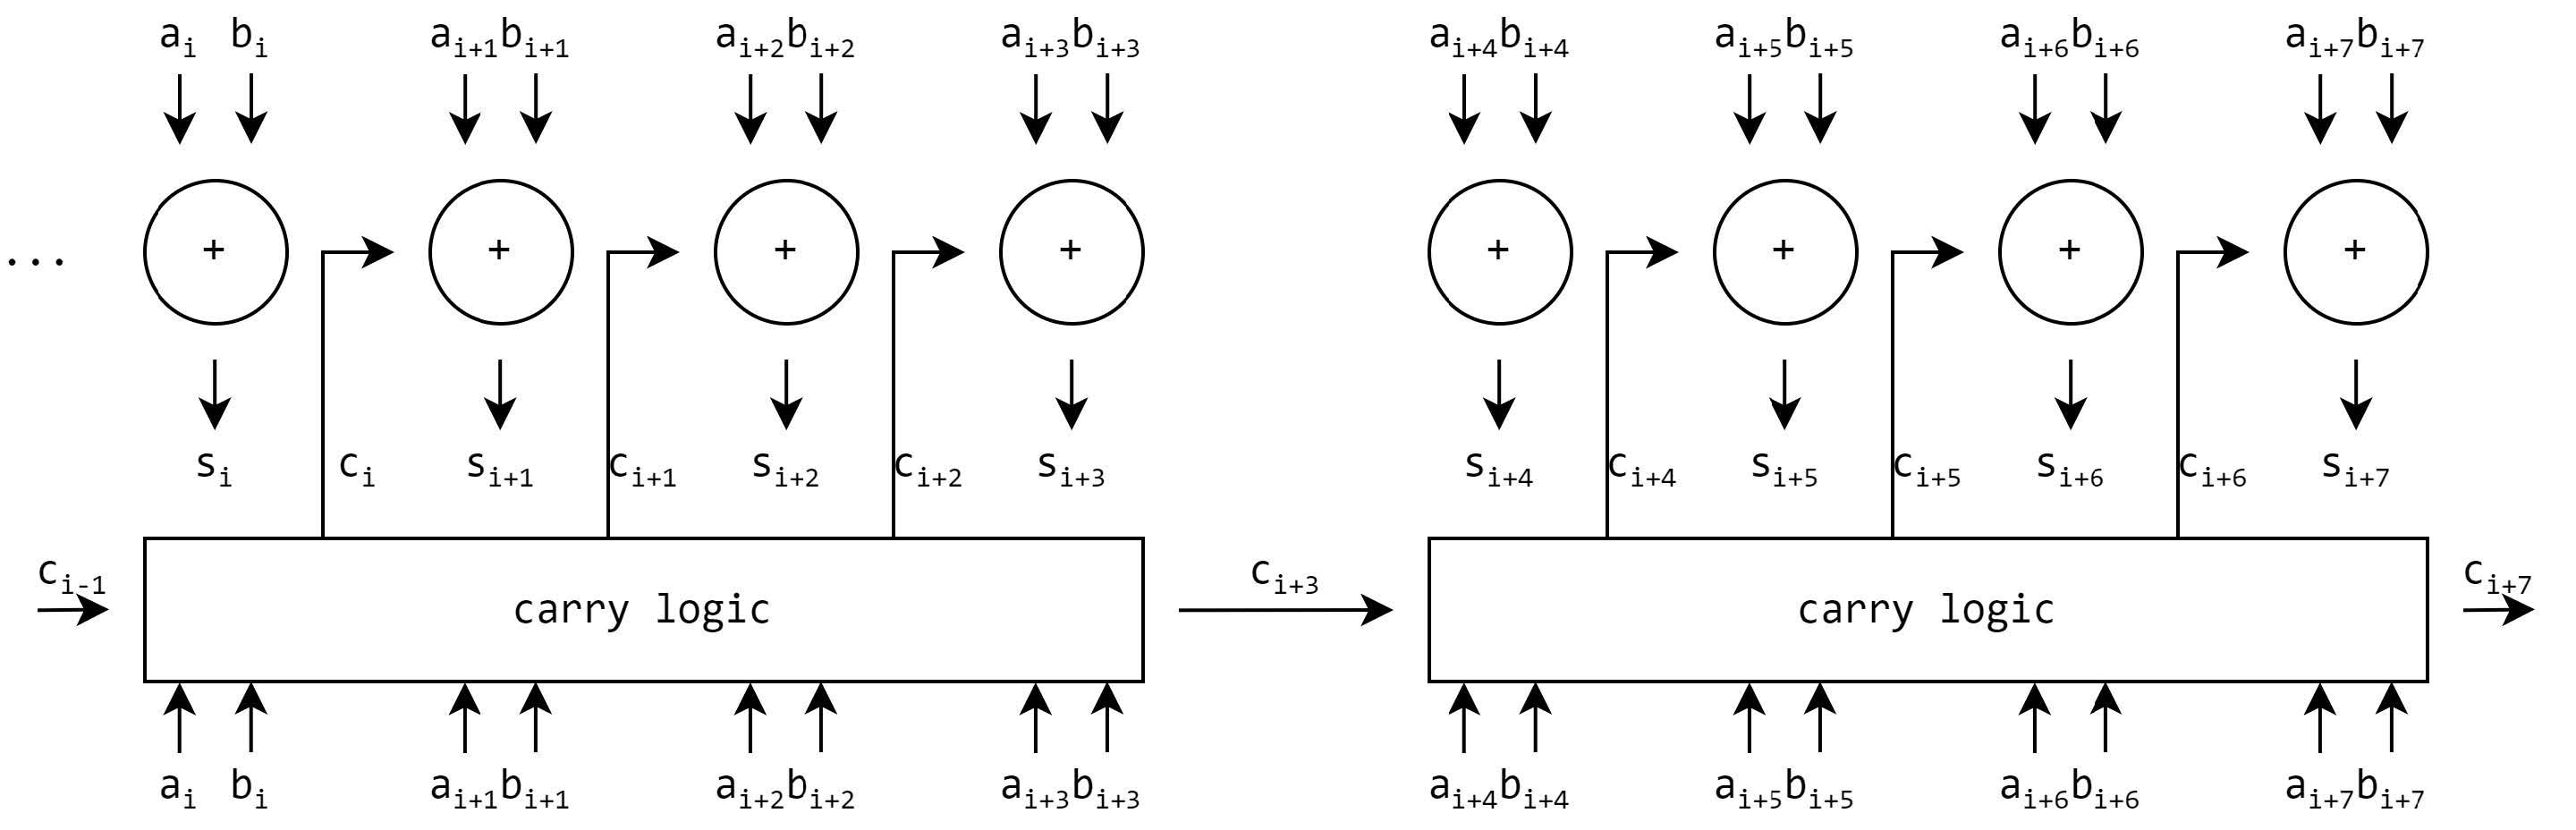
\includegraphics[width=\textwidth]{lab1/6.jpg}
\end{figure}

\subsection{实验内容}

在本节中,您将设计和实现一个8位二进制全加器的Verilog模块,该模块以两个8位二进制数字作为加数输入、一位二进制数字作为进位输入,并输出一个8位二进制数字作为加法结果输出、一位二进制数字作为进位输出。

\textbf{STEP1}:请编写一位二进制全加器的真值表。
\begin{table}[H]
    \centering
    \begin{tabular}{ c c c c c }
        \hline
        \multicolumn{3}{c}{Input} & \multicolumn{2}{c}{Output} \\
        \cmidrule(r){1-3} \cmidrule(r){4-5}
        a & b & $c_{i-1}$ & s & $c_i$ \\
        \hline
        0 & 0 & 0 & 0 & 0 \\
        0 & 0 & 1 & 1 & 0 \\
        \multicolumn{3}{c}{$\cdots$} & \multicolumn{2}{c}{$\cdots$} \\
        \hline
    \end{tabular}
\end{table}

\textbf{STEP2}:请使用Verilog编写一位二进制全加器的代码。
\begin{lstlisting}[language=Verilog]
module bin_adder (
    input a,b,cin,
    output s,cout
);
    // put your code here
endmodule
\end{lstlisting}

\textbf{STEP3}:请使用Verilog编写八位二进制全加器的代码,请实例化您之前编写的一位二进制全加器,自选一种级联方式进行构建,自行仿真测试。\textbf{注意}:出于考察目的,您的任何模块中\textbf{不}应包含“+”运算符。
\begin{lstlisting}[language=Verilog]
module full_adder (
    input [7:0] operand_a,operand_b,
    input carry_in,
    output [7:0] sum,
    output carry_out
);
    // put your code here
    
    // Instantiate your bin_adder, e.g.:
    // bin_adder u_bin_adder (...);
endmodule
\end{lstlisting}

%------------------------------%

\section{上板测试}
为了直观地展示您编写的模块,我们提供了一个测试模块,用以在FPGAOL平台上或您的开发板上驱动外设,其结构如图所示。该测试模块的主要功能是:
\begin{itemize}
    \item 使用定义好的八位二进制全加器接口,实现一个计数器,进行自增或自减计数。
    \item 使用定义好的七段数码管译码器接口,与FPGAOL平台的用户接口进行适配。
\end{itemize}

\begin{figure}[H]
    \centering
    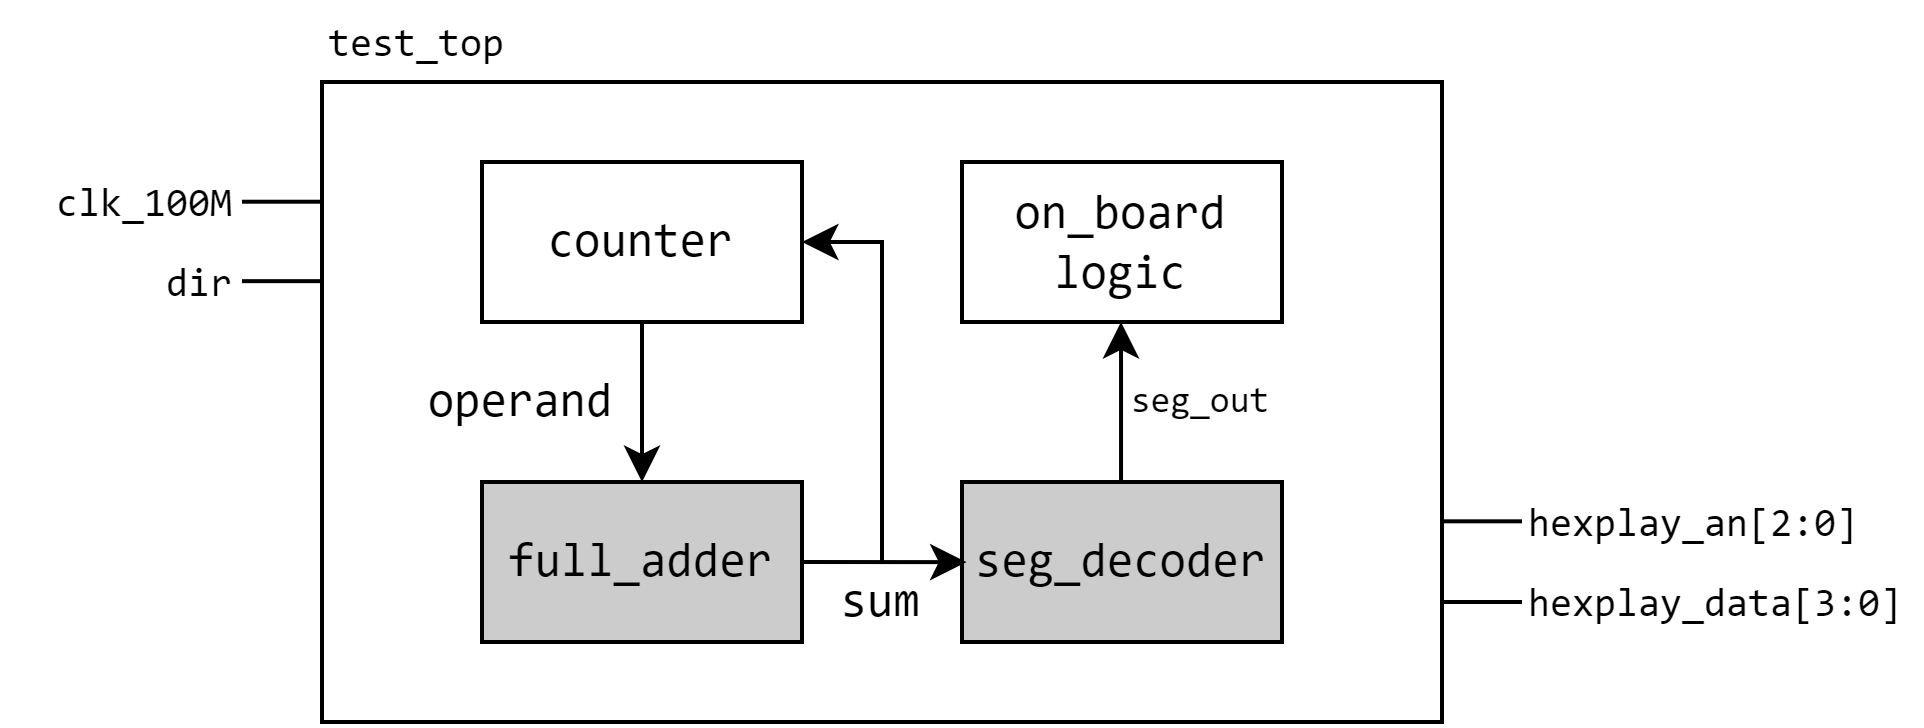
\includegraphics[width=0.65\textwidth]{lab1/7.png}
\end{figure}

请在您创建的工程项目中导入我们的测试文件(见附件test\_top.v)和相应的约束文件(见附件fpgaol.xdc),并在测试文件中补充您在第一节和第二节中所写的Verilog模块。

所有代码编写完成后,使用Vivado完成代码的\underline{综合、实现、生成比特流}的操作,并将生成的比特流上传到FPGAOL平台或自己的板卡上进行测试。在FPGAOL平台上的展示效果如图所示。

\begin{figure}[H]
    \centering
    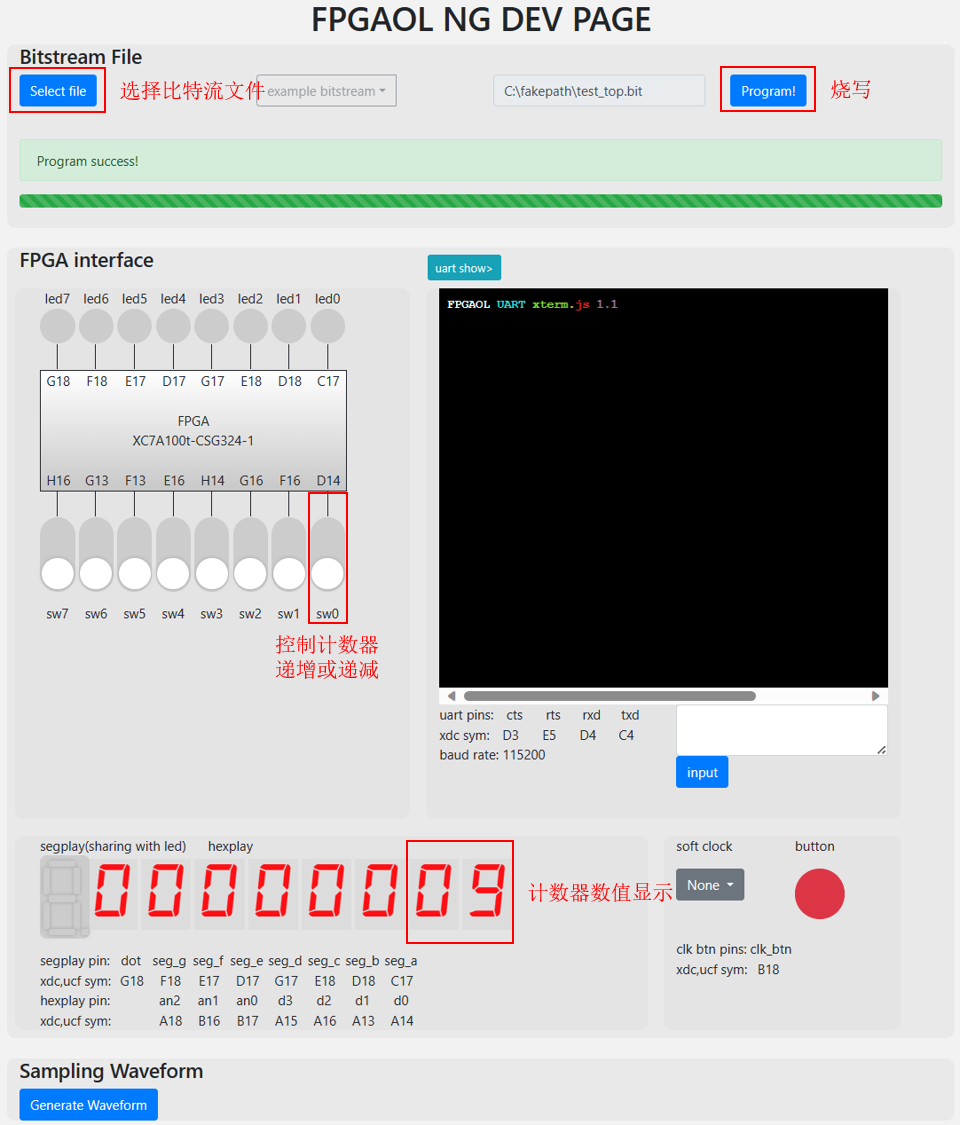
\includegraphics[width=0.65\textwidth]{lab1/8.png}
\end{figure}

%------------------------------%
\section{附件}

\subsection{test\_top.v}
\begin{lstlisting}[language=Verilog]
`timescale 1ns / 1ps

module test_top(
	input CLK100MHZ,
	input dir,
	output reg [2:0] hexplay_an,
	output reg [3:0] hexplay_data
);

reg [31:0] data;
reg [32:0] hexplay_cnt;
reg [ 3:0] hexplay_sel;

always@(posedge CLK100MHZ) begin
	if (hexplay_cnt >= (2000000 / 8))
		hexplay_cnt <= 0;
	else
		hexplay_cnt <= hexplay_cnt + 1;
end

always@(posedge CLK100MHZ) begin
	if (hexplay_cnt == 0)begin
		if (hexplay_an == 7)
			hexplay_an <= 0;
		else
			hexplay_an <= hexplay_an + 1;
	end
end

always@(*) begin
	case(hexplay_an)
		0: hexplay_sel = data[3:0];
		1: hexplay_sel = data[7:4];
		2: hexplay_sel = data[11:8];
		3: hexplay_sel = data[15:12];
		4: hexplay_sel = data[19:16];
		5: hexplay_sel = data[23:20];
		6: hexplay_sel = data[27:24];
		7: hexplay_sel = data[31:28];
	endcase
end

reg [26:0] timer_cnt;
always@(posedge CLK100MHZ) begin
	if (timer_cnt >= 100000000)
		timer_cnt <= 0;
	else
		timer_cnt <= timer_cnt + 1;
end

wire [7:0] data_sum;
wire data_carry;
full_adder u_full_adder (data[7:0], dir ? 8'hff : 8'h01, 1'b0, data_sum, data_carry);

always@(posedge CLK100MHZ) begin
	if (timer_cnt == 0) begin
		data <= data_sum;
	end
end

wire [6:0] seg_wire;
seg_decoder u_seg_decoder (hexplay_sel, seg_wire);

always @(seg_wire) begin
	case (seg_wire)
		7'b0000001: hexplay_data = 4'h0;
		7'b1001111: hexplay_data = 4'h1;
		7'b0010010: hexplay_data = 4'h2;
		7'b0000110: hexplay_data = 4'h3;
		7'b1001100: hexplay_data = 4'h4;
		7'b0100100: hexplay_data = 4'h5;
		7'b0100000: hexplay_data = 4'h6;
		7'b0001111: hexplay_data = 4'h7;
		7'b0000000: hexplay_data = 4'h8;
		7'b0000100: hexplay_data = 4'h9;
		7'b0001000: hexplay_data = 4'ha;
		7'b1100000: hexplay_data = 4'hb;
		7'b0110001: hexplay_data = 4'hc;
		7'b1000010: hexplay_data = 4'hd;
		7'b0110000: hexplay_data = 4'he;
		7'b0111000: hexplay_data = 4'hf;
		default: hexplay_data = 4'h0;
	endcase
end

endmodule

module seg_decoder (
    input [3:0] hex_in,
    output [6:0] seg_out // a-g
);
    // put your code here.
endmodule

module bin_adder (
	input a,b,cin,
    output s,cout
);
    // put your code here
endmodule

module full_adder (
    input [7:0] operand_a,operand_b,
    input carry_in,
    output [7:0] sum,
    output carry_out
);
    // put your code here
    // Instantiate your bin_adder, e.g.:
    // bin_adder u_bin_adder (...);
endmodule
\end{lstlisting}

\subsection{fpgaol.xdc}
\begin{lstlisting}
## Clock signal
set_property -dict { PACKAGE_PIN E3 IOSTANDARD LVCMOS33 } [get_ports { CLK100MHZ }];
create_clock -add -name sys_clk_pin -period 10.00 -waveform {0 5} [get_ports { CLK100MHZ }];

##Switches

set_property -dict { PACKAGE_PIN D14 IOSTANDARD LVCMOS33 } [get_ports { dir }];

##7-Segment Display

set_property -dict { PACKAGE_PIN A14 IOSTANDARD LVCMOS33 } [get_ports { hexplay_data[0] }];
set_property -dict { PACKAGE_PIN A13 IOSTANDARD LVCMOS33 } [get_ports { hexplay_data[1] }];
set_property -dict { PACKAGE_PIN A16 IOSTANDARD LVCMOS33 } [get_ports { hexplay_data[2] }];
set_property -dict { PACKAGE_PIN A15 IOSTANDARD LVCMOS33 } [get_ports { hexplay_data[3] }];
set_property -dict { PACKAGE_PIN B17 IOSTANDARD LVCMOS33 } [get_ports { hexplay_an[0] }];
set_property -dict { PACKAGE_PIN B16 IOSTANDARD LVCMOS33 } [get_ports { hexplay_an[1] }];
set_property -dict { PACKAGE_PIN A18 IOSTANDARD LVCMOS33 } [get_ports { hexplay_an[2] }];
\end{lstlisting}

\end{document}